\documentclass[11pt, letterpaper, titlepage]{article}
\usepackage[utf8]{inputenc}
\usepackage{geometry}
\usepackage{color,graphicx,overpic} 
\usepackage{fancyhdr}
\usepackage{amsmath,amsthm,amsfonts,amssymb}
\usepackage{mathtools}
\usepackage{hyperref}
\usepackage{multicol}
\usepackage{array}
\usepackage{float}
\usepackage{blindtext}
\usepackage{longtable}
\usepackage{scrextend}
\usepackage[font=small,labelfont=bf]{caption}
\usepackage[framemethod=tikz]{mdframed}
\usepackage{calc}
\usepackage{titlesec}
\usepackage{listings}
\usepackage[normalem]{ulem}
\usepackage{tabularx}
\usepackage{mathrsfs}
\usepackage{bookmark}
\usepackage{setspace}
\usepackage{tabularx}
\usepackage{ltablex}
\usepackage{enumitem}
\usepackage{minted}
\usepackage[simplified]{pgf-umlcd}
\usepackage{apple_emoji}

\mathtoolsset{showonlyrefs}  
\allowdisplaybreaks
\definecolor{mycolor}{rgb}{0, 0, 0}

\geometry{top=2.54cm, left=2.54cm, right=2.54cm, bottom=2.54cm}
\setlength{\headheight}{20pt}
\setlength{\parskip}{0.5cm}
\setlength{\parindent}{0pt}

\newcolumntype{s}{>{\hsize=.25\hsize}X}
\newcolumntype{m}{>{\hsize=.6\hsize}X}

\definecolor{bg}{rgb}{0.95,0.95,0.95}

\usemintedstyle{vs}
\setminted{linenos, fontsize=\footnotesize}
\setmintedinline{bgcolor=bg, style=bw, fontsize=\normalsize}

% Line spacing
\renewcommand{\baselinestretch}{1.3} 

% Title page
\title{\textbf{\Huge{ 
\begin{center}
ECE 315 Lab 3 🧀
\end{center} 
}}}

\author{For Ahmed and Shyama 🎁💯🙏 \\ \\ 🚙 Lora Ma \\ 🌎 Benjamin Kong \\ \\ECE 315 Lab Section H41}

% Header/Footer
\pagestyle{fancy}
\fancyhf{}
\rhead{\thepage}
\lhead{\textit{ECE 315 - Lab 3}}
\rfoot{}

% Hyperlink colors
\hypersetup{
    colorlinks=true,
    linkcolor=blue,
    filecolor=blue,      
    urlcolor=blue,
}

\begin{document}
\maketitle
\thispagestyle{empty}
\tableofcontents 
\newpage
\pagenumbering{arabic}

\section{Abstract}
The purpose 🔬💯 of this lab was to 
\begin{itemize}
  \item gain experience using the serial peripheral interface in both the master and slave modes
  \item gain experience creating artificial load on a CPU and then measuring the resulting load using \mintinline{text}{vTaskGetRunTimeStats()}.
\end{itemize}
We will be using the 🎱 Zybo Z7 development board by 🚰 Digilent. The 🧀 board is built around the Xilinx Zynq-7010 System-on-Chip silicon chip and contains two 667 MHz ARM Cortex A9 32-bit CPUs. For this lab, we will be using CPU0 to run the FreeRTOS real-time kernel which will have three non-idle 💤 tasks for the SPI interface. 

In this 🚀 lab, we will be completing two exercises. Exercise 🏆 1 is to verify the given system and add the byte count message. The program will echo characters that are type on the keyboard until the termination sequence \mintinline{text}{\r#\r} is detected. Then, a string will be generated and sent over SPI which will look something like \mintinline{text}{The number of characters received over SPI: <number> \n} where \mintinline{text}{<number>} is the total bytes that were received over the SPI1 interface.

In exercise 🎯 2, we will be calibrating the load generator experimentally. The program prints the percentage values of time consumed by the tasks \mintinline{text}{TaskCPULoadGen}, \mintinline{text}{TaskLoopCountProcessor}, and \mintinline{text}{TaskPrintRunTimeStats}. It will be displayed in a tabular format on the terminal. We will the utilize this program to experimentally determine the value of \mintinline{text}{loop_count}. 

\section{Design}

\subsection{Exercise 1 Design}
A systematic diagram that illustrates the relationship between the SDK terminal on the host, the UART interface, the SPI0 and SPI1 interfaces, and the three tasks is shown below. 🍅
\begin{figure}[H]
    \centering
    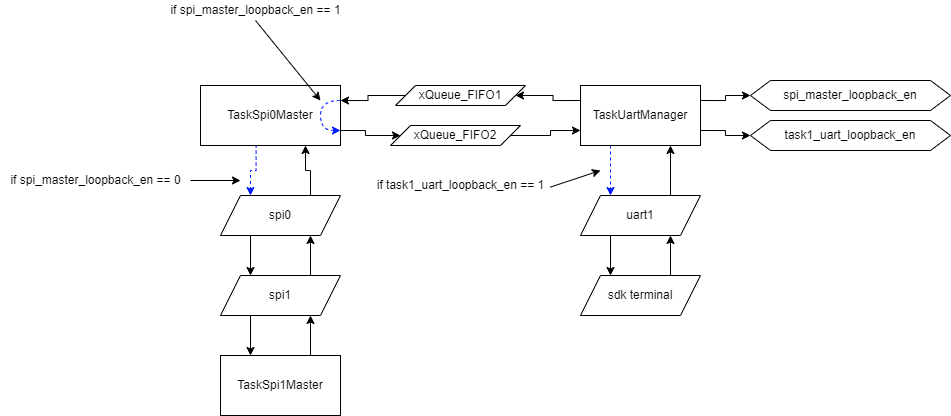
\includegraphics[width=\textwidth]{Diagram.png}
    \caption{Systematic diagram showing the connections between each element.}
\end{figure}
Below, the 😤 block design for this exercise is shown. The 😤 confections between SPI0 and SPI1 are clearly visible. For example, \mintinline{text}{SPI0_MOSI_I} is connected to \mintinline{text}{SPI1_MOSI_O}, \mintinline{text}{SPI0_MOSI_O} is connected to \mintinline{text}{SPI1_MOSI_I}, \mintinline{text}{SPI0_MISO_I} is connected to \mintinline{text}{SPI1_MISO_O}, and \mintinline{text}{SPI0_MISI_O} is connected to \mintinline{text}{SPI1_MISO_I}.
\begin{figure}[H]
    \centering
    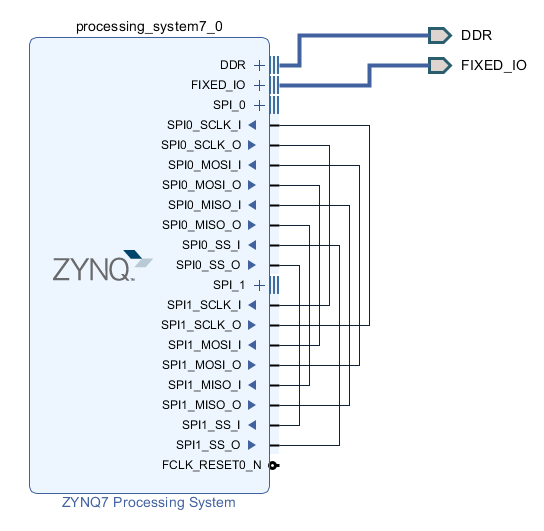
\includegraphics[width=0.6\textwidth]{Diagram2.png}
    \caption{Block design for this exercise.}
\end{figure}

In exercise 1, we first completed the \mintinline{text}{TaskUartManager} function. We wrote the logic to send a dummy character using FIFO1 and then receive the bytes from FIFO2 once the \mintinline{text}{TaskSpi0Master} responds. 💰

The second thing we completed was the \mintinline{text}{TaskSpi0Master} function. We first copy the received data from FIFO1 into a buffer. We transfer bytes based on the \mintinline{text}{TRANSFER_SIZE_IN_BYTES} value. For this lab, the value was set to 1 (i.e. 1 byte). We use the \mintinline{text}{bytecount} variable to keep track of how many bytes we have stored in the buffer and compare it to \mintinline{text}{TRANSFER_SIZE_IN_BYTES} to determine if we need to sent the data yet.

Once we have determined we need to transfer, we call \mintinline{text}{SpiMasterWrite} to transfer the bytes to the slave. We then call \mintinline{text}{taskYIELD()} to allow the slave to work. Once the slave yields back to this task, we read data from master into \mintinline{text}{send_SPI_data_via_FIFO2} (this variable is a variable to help us store intermediary results). We then send this to data to the back of FIFO2. Lastly, we reset \mintinline{text}{bytecount} back to 0 to allow data to accumulate in the buffer again before repeating this whole process again.

The last function we completed was the \mintinline{text}{TaskSpi1Slave} function. We wrote logic to detect the termination sequence \mintinline{text}{\r#\r}. This was done by incrementing the \mintinline{text}{end_sequence_flag} variable whenever the correct termination character appeared and resetting it to 0 otherwise. If the flag reached 3 (the length of \mintinline{text}{\r#\r}) then we proceed to the logic for handling termination.

Our goal when the termination sequence is triggered is to send the bytes that make up the message ``The number of characters received over SPI:\%d'' to the master SPI. In order to do this, we set the \mintinline{text}{flag} variable to 1 and then used a for loop to send the bytes. This is done by using \mintinline{text}{SpiSlaveWrite} and sending 1 byte. We then use \mintinline{text}{SpiSlaveRead} to receive the response. Once all the bytes have been sent by using the for loop, we reset our counters/flags to allow this process to repeat.

\subsection{Exercise 2 Design}
In exercise 2, we attempted to find values of \mintinline{text}{loop_count} that result in 90\%, 80\%, 70\%, 60\%, 50\%, and 40\% idle load percentages. In order to do this, we completed the necessary functions and testing varying values of \mintinline{text}{loop_count} until we found the desired idle load percentages. The table below shows the values of \mintinline{text}{loop_count} that resulted in the aforementioned idle load percentages. 🍞
\begin{tabularx}{\textwidth}{|X|X|X|X|X|X|X|}
    \caption{\mintinline[fontsize=\small]{text}{loop_count} values for the corresponding idle load percentages} \\
    \hline
    Load & 90\% & 80\% & 70\% & 60\% & 50\% & 40\%  \\ \hline
    Loop count & 50000 & 125000 & 200000 & 275000 & 350000 & 400000 \\ \hline
\end{tabularx}

For \mintinline{text}{TaskLoopCountProcessor}, we set the \mintinline{text}{delay} variable to 90000 ms if \mintinline{text}{loop_count} exceeded 500000 and 120000 ms if \mintinline{text}{loop_count} exceeded 1000000. We also incremented the \mintinline{text}{loop_count} variable by 25000 for each loop. 

For the \mintinline{text}{TaskCpuLoadGen} function, we needed something to execute to simulate CPU load. To do this, we iterated \mintinline{text}{loop_count} number of times, each time taking the bitwise complement of a dummy variable. This was done via \mintinline{text}{var = !var}.

Lastly, for the \mintinline{text}{TaskPrintRunTimeStats} function, we needed to output the runtime stats using \mintinline{text}{vTaskGetRunTimeStats}. We first enabled this feature as described in the helper document. We then created a character buffer and wrote the runtime stats into the buffer using \mintinline{text}{vTaskGetRunTimeStats}. We then used \mintinline{text}{xil_printf} to output the buffer which contains the runtime stats.

\section{Testing}
(yeet 🚗 vroom 🚕 vroom 🚙 car go 💨 brrrrr)
\subsection{Exercise 1 Tests}
\begin{tabularx}{\textwidth}{|X|X|m|}
  \caption{Tests for exercise 1.} \\
  \hline
  \textbf{Description} & \textbf{Expected} & \textbf{Pass} \\ \hline
  Enter ``12345'' in initial menu & Nothing appears & Yes \\ \hline
  Enter ``1'' in the initial menu & UART Manager Task loopback enabled & Yes \\ \hline
  In task1 loopback mode: enter ``12345'' & ``12345'' appears in terminal & Yes \\ \hline
  In task1 loopback mode: enter ``Ben'' & ``Ben'' appears in terminal & Yes \\ \hline
  In task1 loopback mode: enter ``1'' & UART Manager Task loopback disabled using command toggling & Yes \\ \hline
  Then enter ``12345'' & Nothing appears & Yes \\ \hline
  Then enter ``1'' & UART Manager Task loopback enabled & Yes \\ \hline
  In task1 loopback mode: enter ``12345'' & ``12345'' appears in terminal & Yes \\ \hline
  Then enter ``\#'' & UART Manager Task loopback disabled using termination sequence & Yes \\ \hline
  Then enter ``12345'' & Nothing appears & Yes \\ \hline
  Then enter ``2'' & Task2 loopback enabled: No access to SPI0 interface & Yes \\ \hline
  In task1 loopback mode: enter ``12345'' & ``12345'' appears in terminal & Yes \\ \hline
  In task1 loopback mode: enter ``Ben'' & ``Ben'' appears in terminal & Yes \\ \hline
  Then enter ``2'' & Task2 loopback disabled using command toggling: SPI0-SPI1 in effect. Send the bytse from the console & Yes \\ \hline
  In task1 loopback mode: enter ``Benjamin'' & ``[]Benjamin'' appears in terminal & Yes \\ \hline
  Then enter ``\#'' & The number of characters received over SPI:8 & Yes \\ \hline
  In task1 loopback mode: enter ``Yeet'' & ``[]Yeet'' appears in terminal & Yes \\ \hline
  Then enter ``\#'' & The number of characters received over SPI:4 & Yes \\ \hline
\end{tabularx}

\section{Conclusion}
The purpose of this lab was to 
\begin{itemize}
  \item gain experience using the serial peripheral interface in both the master and slave modes
  \item gain experience creating artificial load on a CPU and then measuring the resulting load using \mintinline{text}{vTaskGetRunTimeStats()}. 💰💰💰
\end{itemize}

We believe we have fully completed the objectives of this lab. 🚒

In exercise 1, we gained experience using the SPI interface. The program echos characters that are typed on the keyboard until the termination sequence is detected. Then, it will generate a string to be sent over SPI where it will print the number of total bytes that were received over the SPI interface. 🍕

In exercise 2, we created a program that prints the percentage values of time consumed by three tasks. We summarized this information to be printed in a tabular format in the terminal. This program was then used to experimentally determine the value of \mintinline{text}{loop_count}. 😐😷

We were able to gain experience using the serial peripheral interface (SPI) in both master and slave modes. We were also able to gain experience creating artificial load on a CPU and then measuring the resulting load using \mintinline{text}{vTaskGetRunTimeStats()}. 🚒

\section{Appendix}

\subsection{Exercise 1 Source Code}
The source code is in the file \mintinline{text}{spi_lab3_main.c} that was submitted along with this report. 💵💵💵

\subsection{Exercise 2 Source Code}
The source code is in the file \mintinline{text}{load_gen_main.c} that was submitted along with this report. 💵💵💵

\end{document}